\documentclass{article} % For LaTeX2e
\usepackage{cos424,times}
\usepackage{url}
\usepackage{graphicx}
\usepackage{hyperref}
\usepackage{caption}
\usepackage{subcaption}
\usepackage{amsmath}
\usepackage{amssymb}

\title{Netflix Genre-Based Movie Prediction}


\author{
Gregory McCord\\
Princeton University '20\\
\texttt{gmccord@princeton.edu} \\
}

\newcommand{\fix}{\marginpar{FIX}}
\newcommand{\new}{\marginpar{NEW}}

\begin{document}

\maketitle

\begin{abstract}

Over the past 5 years, Netflix has grown from having 26.5 million subscribers in 2012 to having 117.6 million subscribers in the first quarter of 2018 \cite{view}. Accordingly, their net worth just hit a milestone, with the value of the company reaching \$100 billion this year, cementing itself as the premier source for streaming video \cite{money}. With so many subscribers, Netflix must maintain their vast movie collection and predict what movies and shows a user would like based on their specific set of preferences, which can be complicated since many users do not have many data points. Since Netflix offers tens of thousands of movies and shows to its millions of subscribers, the prediction matrix is inherently sparse, but the issues outlined prior contribute to the difficulty of accurately predicting movies that users will want to watch. For this assignment, we used the official Netflix Prize competition dataset consisting of 2,649,430 users' star ratings (out of 5) for 17,770 movies. We reduced the dimensionality of the data by removing users with a small number of movies watched and movies with few ratings. We used a combination of the users' ratings of the movies and the genres of the movies to predict whether or not a user would like a movie. Our baseline implementation performed logistic regression on each individual to determine if they would like or dislike each each movie. Additionally, we used coordinate descent to optimize hyperparameters while determining point estimates for the latent factors that characterize each movie. In our study, the coordinate descent approach obtained small improvements in classification rate over basic logistic regression on out-of-sample test cases.

\end{abstract}

\section{Introduction}

The problem, as tasked, was to identify a trend in the Netflix data and predict as accurately as possible the ratings from users on unobserved data points. These missing data points could be considered in several ways. With no imputation, all non-rated movies would be treated as 0s on a scale of 0-5, indicating that the user intentionally did not watch the movies. Alternatively, these values could represent a mixture of movies that the user has not gotten around to watching but might like and movies that the user actively chose not to watch. Netflix and other streaming services value accurate predictions of these missing labels because it helps to provide users with content that draws them in and entices them to continue their subscription (in the case of Netflix) or continue to view their content (in the case of YouTube). Our study in particular attempts to classify these labels using genre data available from IMDb augmented with collaborative filtering, an approach which has not been used before.

We tested two different models in this study. First, we performed logistic regression on each individual, using the user's rating labels as the response variable and the genre data as the features. Next, we took an iterated approach using coordinate descent to factor in latent variables to the model. By iteratively holding different variables constant, we were able to maximize the log-likelihood of the function and minimize the misclassification rate. Our methods performed very well on the datasets, with the misclassification rate over all withheld points resting around 18\% for both methods with coordinate descent performing better. First, we will describe the motivation behind our approach. Then, we will describe the methodology and metrics used in our analysis, followed by a detailed description of our coordinate descent algorithm. Finally, we will analyze the results, discuss the overall project, and propose steps for moving forward.

\section{Related Work}

This dataset was released by Netflix for their Netflix Prize competition that was launched in 2006 and concluded in 2009. The prize was awarded to the BellKor's Pragmatic Chaos, which significantly outperformed the previous techniques used by Netflix at the time. Their solution utilized user ratings and date-stamped movie ratings (which were present in the original competition dataset) to accurately predict which movies and shows a particular user would like and dislike. Their specific solution used a collaborative filtering system that implemented a number of predictors including many advanced models such as Restricted Boltzmann Machines and gradient boosted decision trees \cite{bellkor}. While this and many other solutions attacked the problem using strictly the rating and time data, we attempted to create a collaborative filter to predict a users preferences using genre data, an approach that does not seem to have been used before.

\section{Methods}

The original data was provided to us in a scipy sparse matrix \cite{scipy} along with a list of movies and their years of production. In addition to this, we used the IMDbPY Python3 library to obtain the genre data on as many of these movies as possible \cite{imdb}. We were able to obtain genre data for most movies in the list, but several items such as "Lord of the Rings: The Return of the King: Extended Edition: Bonus Material" were not found in IMDb and were therefore removed from the dataset. Our data therefore consisted of 2 matrices. One represented the users' ratings of movies while the other represented the genre data of each movie.

\subsection{Data Processing}

Referenced briefly above, we eliminated the rows in each matrix which we were not able to pull data for from IMDb. Additionally, we found the sum of each column and row individually, and sorted both lists. We plotted them versus their sorted index in figures \ref{fig:sub1} and \ref{fig:sub2}. We selected the threshold for movies as the value of the movie at index 2,500 (since it is near where the asymptotic behavior begins) and performed the same process on viewers using index 100,000.

\begin{figure}[htb]
\centering
\begin{subfigure}{.5\textwidth}
  \centering
  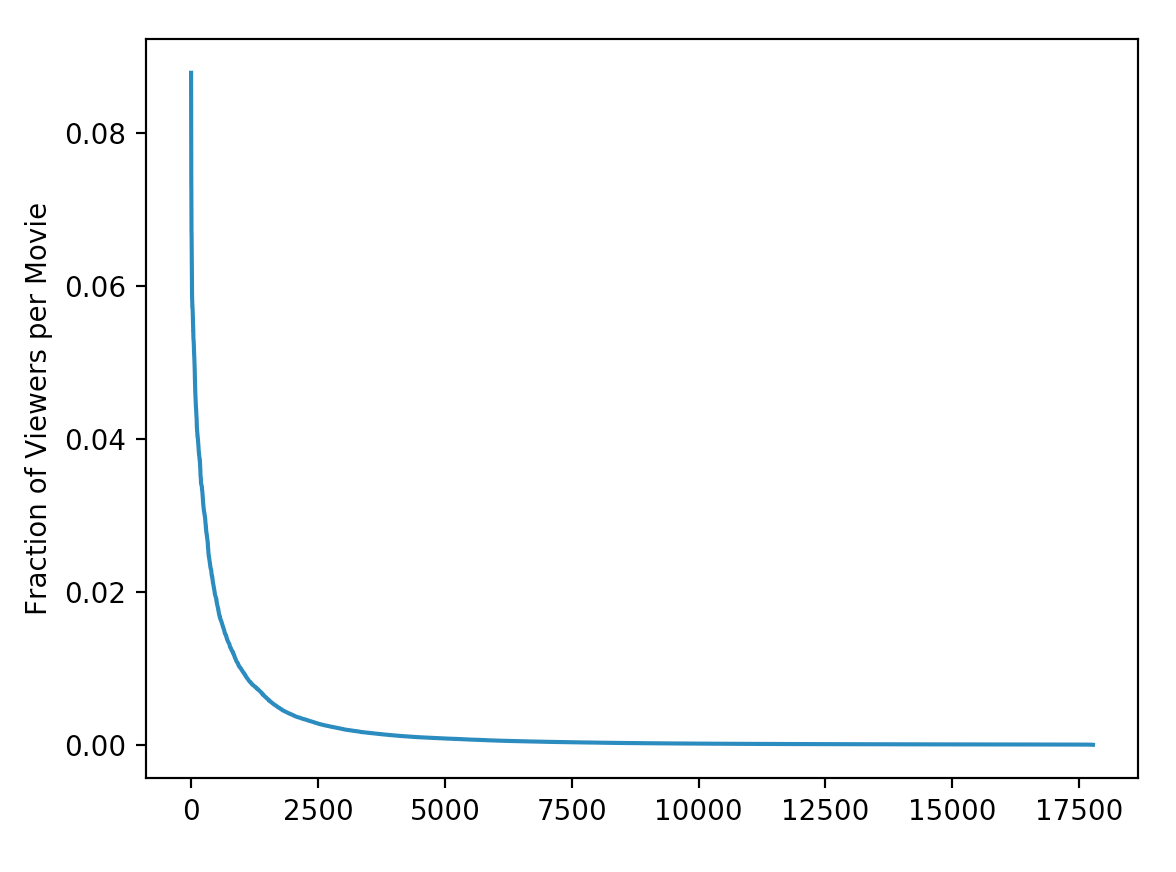
\includegraphics[width=.9\linewidth]{movies_by_views}
  \caption{Movies by number of views}
  \label{fig:sub1}
\end{subfigure}%
\begin{subfigure}{.5\textwidth}
  \centering
  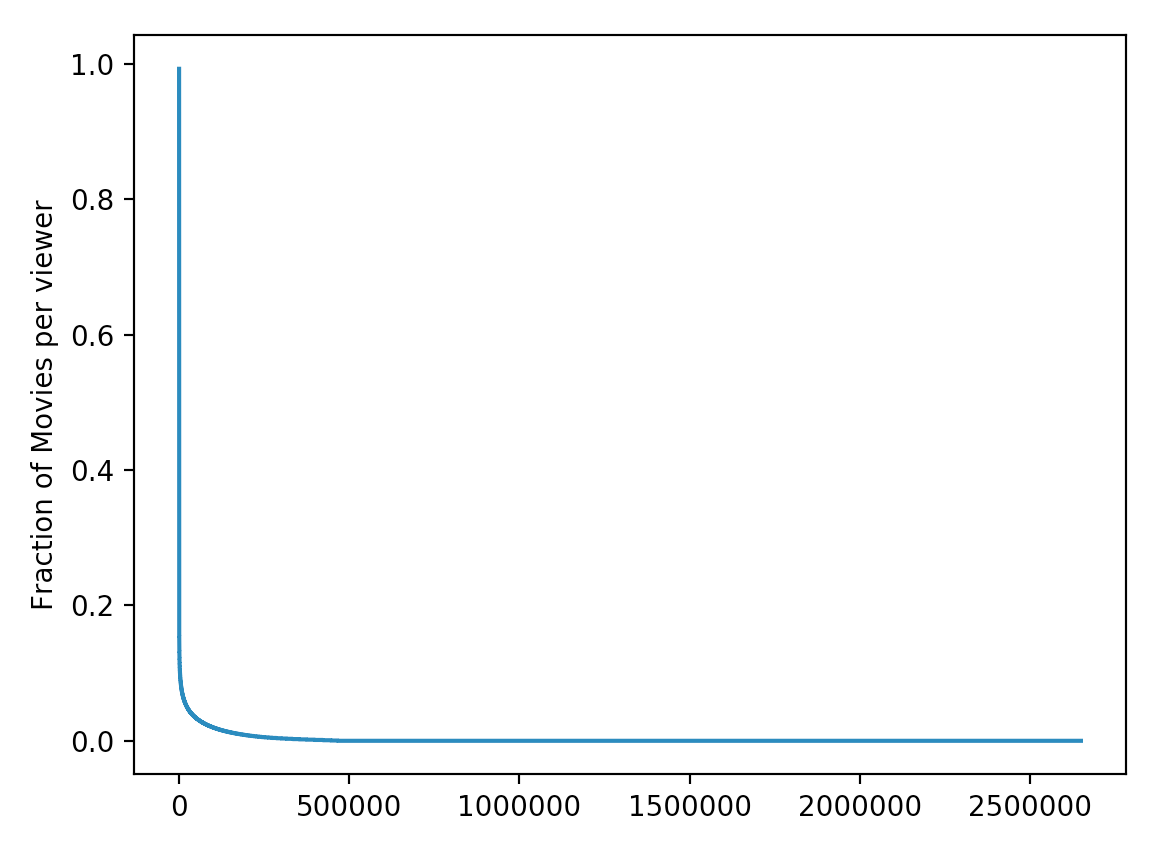
\includegraphics[width=.9\linewidth]{users_by_ratings}
  \caption{Users by number of movies rated}
  \label{fig:sub2}
\end{subfigure}
\end{figure}

After these steps, we were left with 2,384 movies and approximately 100,000 users with approximately 10\% of the ratings known. To turn this into a binary classification problem to reduce the complexity of the model to whether a user would like or dislike a movie (where a rating of 1 or 2 indicated dislike). However, issues arose since many users primarily gave positive or negative ratings. We created a test test that randomly selected 1\% of the data points from each user and hid the true value such that the algorithm would treat the rating as unobserved and attempt to predict it. We had to iteratively remove users until there were 9,810 users remaining, all of whom rated many movies but showed some differentiation in terms of preference for movies they had seen. This binary matrix consisted of 2,194,191 known entries, from which we randomly selected 16,357 (approximately 1\%) observations to hide from the algorithms. We set the seed so that the withheld points were the same for all models. After obtaining the genre data and removing the appropriate rows, we performed one hot encoding, which produced a matrix with 27 columns - 1 column per genre.

\subsection{Classification Methods}

We implemented two algorithms for predicting the missing and withheld labels for each viewer. We reduced the problem to binary classification because many viewers have a tendency to rate on the extremes, generating a bimodal distribution. Following this transformation, we used the scikit-learn Python library to perform logistic regression for every user individually \cite{skl}. We trained the model for each user on the specific set of movies that had non-missing, non-withheld labels and used the binary data as the prediction labels. Therefore, the coefficient vector $\beta_j$ for the $j^{th}$ user represent their movie preferences. We did not tune the hyperparameter of the logistic regression model - the inverse of regularization strength parameter, C, was set to 0.2 for most trials and 1.0 for the remaining. We applied $\ell_2$ regularization to the model rather than $\ell_1$ since there were only 27 features in the training set.

We used coordinate descent as a more reformed approach, which was motivated by several facts. First, we wanted to incorporate latent variables to give a two-dimensional characterization of the individual movies, the values of which were learned from the similarities between users. Similar to the EM algorithm, coordinate descent maximizes the log-likelihood (or minimizes the negative log-likelihood) of the observed data and is used to fit the latent variable model. However, our coordinate descent algorithm assigns a binary label to the response variable rather than a probability distribution over the set of labels. We initialized the latent variables by drawing from a normal distribution. In the E step, we generated logistic regression models for each user. In the M step, we learned the values for the latent variables by testing different sets of parameters and taking the maximum log-likelihood subject to $\ell_1$ regularization. See section \ref{cd} for more information on our specific implementation of the algorithm.

\subsection{Evaluation of Results}

To evaluate our results, we calculated the misclassification rate of labels in two ways. First, we compared the predicted labels versus the true labels on the withheld data for each individual user and averaged these ratings across all users. We will refer to this as $MC_1$. Second, we compared the total number of correctly classified labels with the total number of withheld samples. We will refer to this as $MC_2$.
\begin{align*}
MC_1 = 1 - \frac{\sum_j \left( \sum_i C_{i,j} \cdot W_{i,j} / N_j \right)}{U} \hspace{15mm}
MC_2 = 1 - \frac{\sum_j \sum_i C_{i,j} \cdot W_{i,j} }{N}
\end{align*}

where $U$ represents the number of users, $C_{i,j}$ is a binary label representing if the value at $i,j$ was classified correctly, $W_{i,j}$ designates if the label was withheld or not, and $N_j$ is the number of withheld points in column j. Note that $N=\sum_j N_j$ and $C_{i,j} \cdot W_{i,j} = 1$ only if the value was classified correctly and withheld.

\section{Key Algorithm: Coordinate Descent}\label{cd}

Coordinate Descent (Dempster, Laird, Rubin 1977) is an optimization algorithm that attempts to find the set of parameters that minimize the negative log-likelihood by iterating over the data holding different sets of parameters fixed at different moments. While describing the method in the case of our project, let $\mathcal{D} = (\textbf{x}_{i},z_{i,j}) ,  \forall i \in M , j \in U$ where $M$ is the set of movies and $U$ is the set of users. Since in our experiment each user had a different number of movies watched, we will assume that $\mathcal{D}$ has been cleaned such that some labels $z_{i,j}$ could be missing (either unknown or withheld) but all present labels are binary (where 0 represents movies rated a 1 or 2). If this is the case, we simply skip this $i$ for the user $j$ when training the model.

Each label $z_{i,j}$ is modeled as a Bernoulli random variable $X_{i,j}$. For basic logistic regression, this is represented by $X_{i,j} = Ber(S(B_j \cdot x_i + B_0))$ where S is the sigmoid function defined by the following:
\begin{align*}
S(x) = \frac{1}{1+e^{-x}}
\end{align*}

However, because we are including latent factors in our analysis, our parameter random variables becomes $X_{i,j} = Ber(S(B_j \cdot x_i + \alpha_j \cdot y_i + B_0))$. In our experiment, we tested $y_i $ with dimension 1 and 2, but the two-dimensional approach provided more accurate classification. $y_i$ represents the latent variables in the model. These movie constants provide a characterization of the movie that is learned from the preferences of the collective body of users. $\alpha_j$ is analogous to $B_j$ in that they are the user specific coefficients to the latent variables and observed data, respectively.

There are several steps to the iterative process:
\begin{enumerate}
\item Initialize random values for $y_i$  from a standard normal distribution
\item Hold $y_i$ fixed and perform logistic regression to train $B_j,\alpha_j$
\item Hold $B_j,\alpha_j$ fixed and find the $y_i$ such that the log-likelihood is maximized
\item Repeat steps 2-3 until convergence
\end{enumerate}

Step 3 can be performed in a number of ways and generally depends on the number of latent variables. Because our experiment only involved at most 2 latent variables, it was computationally feasible to perform grid search over some set pairs. Models with more complex systems of latent variables might need to use a more advanced gradient descent algorithm to calculate the optimal point estimates for the variables. In either case, the algorithm attempts to maximize the log-likelihood of the set of $y_i$. Additionally, because we are using this to tune $y_i$, we must perform regularization so that the $y_i$ and $\alpha_j$ do not overwhelm the rest of the terms while guaranteeing that there is a unique solution to the set of parameters. $\ell_1$ is commonly chosen for this task and the one used in our model \cite{mlapp}. The likelihood itself can be represented as the product of the pmfs of all Bernoulli random variables $Z_{i,j}$ in the model, but represented in terms of the regularized log-likelihood, it takes the following form:
\begin{align*}
\log \mathcal{L} = \sum_i \left( \sum_j \log(\hat{p}^{Z_{i,j}}(1-\hat{p})^{1-Z_{i,j}}) - \lambda_{\alpha} ||\alpha_j||_2 - \lambda_B ||B_j||_2 - \lambda ||y_i||_1 \right)
\end{align*}

where $\hat{p} = S(B_j \cdot x_i + \alpha_j \cdot y_i + B_0)$.

Much like with Expectation Maximization, this solution is guaranteed to converge because the objective function (the log-likelihood) has an upper bound, and every iteration strictly increases the value of the log-likelihood. However, the likelihood function could have multiple local maxima, so the algorithm could get caught in a local minima. As such, it is common practice to re-run the model multiple times with different randomly generated starting points.

\section{Results}

To analyze our results, we used two forms of the misclassification rate. $MC_1$ refers to averaging the misclassification rates of all users while $MC_2$ refers to the misclassification rate of the aggregate of all points. While $MC_2$ gives a better out of sample estimate for the number of missing rating labels that can be accurately predicted, $MC_1$ weights each user evenly, which reduces the effect of users with high number of views that would overwhelm the more difficult to predict samples (those for users with fewer data points to predict on). We believed that this estimate would help to differentiate standard logistic regression, which treated all users as independent, from coordinate descent, which factored in latent variables learned from other users.

\begin{figure}[htb]
\centering
\begin{subfigure}{.5\textwidth}
  \centering

\begin{tabular}{|c|c|c|c|} 
\hline
Method & $C$ & $MC_1$ & $MC_2$ \\
\hline\hline
LR & 1 & 0.255 & 0.181 \\
\hline
CD & 1 & 0.250 & 0.178 \\
\hline
LR & 0.2 & 0.249 & 0.180 \\
\hline
CD & 0.2 & \textbf{0.248} & \textbf{0.177} \\
\hline
\end{tabular}
\caption{\textbf{Model results for Logistic Regression (LR) and Coordinate Descent (CD).} C refers to the inverse regularization hyperparameter while $MC_1$ and $MC_2$ are defined as before.}
\label{fig2:sub1}
\end{subfigure}%
\begin{subfigure}{.5\textwidth}
  \centering
  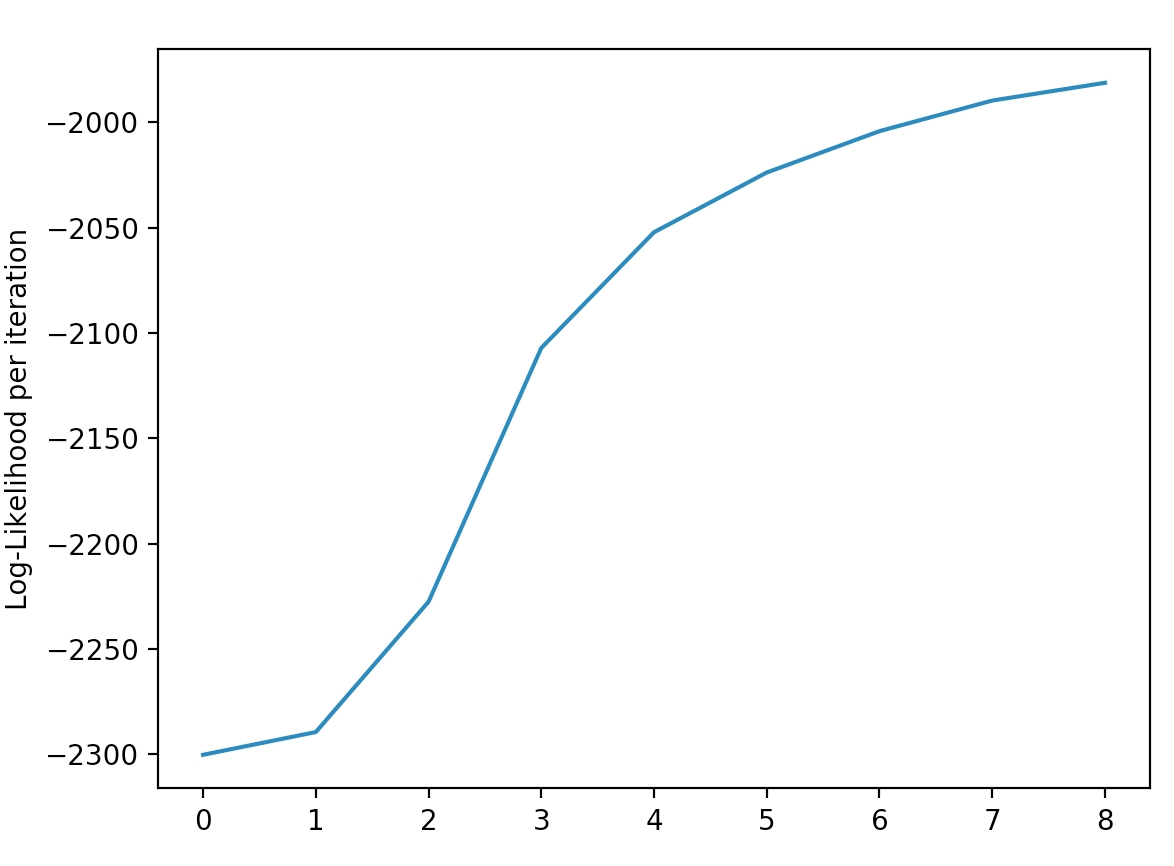
\includegraphics[width=0.9\linewidth]{log-likelihood}
  \caption{Maximum log-likelihood at each iteration}
  \label{fig2:sub2}
\end{subfigure}
\caption{Results of logistic regression and the iterative steps of coordinate descent}
\vspace*{-5mm}
\end{figure}

As seen in \ref{fig2:sub1}, both models performed similarly under all circumstances. The best classification rates obtained in all instances were by the coordinate descent algorithm, but practically there was little differentiation between the two models. Two values of note in particular are the minimum misclassification rates, both obtained by the coordinate descent algorithm with hyperparameter $C=0.2$. In figure \ref{fig2:sub2}, we can see a plot of the likelihood function estimates per iteration for one trial for the model with $C=0.2$. We will use the two sample proportion test with $H_0: p_1-p_2 = 0$:
\begin{align*}
Z = \frac{\hat{p}_1 - \hat{p}_2}{\hat{p}(1 - \hat{p})(\frac{1}{n_1} + \frac{1}{n_2})}
\end{align*}

where $\hat{p} = \frac{\hat{p}_1 n_1 + \hat{p}_2 n_2}{n_1 + n_2}$ represents the fraction of total successes to compare models. While this method shows that the difference between the two methods is not statistically significant ($p\text{-value} = 0.47 > 0.05 = \alpha$), it makes several broad assumptions, particularly of the independence of users, which is contradictory to the assumptions of our model - that collaborative filtering helps us to better predict ratings. As such, while this gives us an idea of the comparison between the methods and should be included for completeness, the inference is not perfect and is likely incorrect in practice.

\section{Discussion and Conclusion}

By observing the magnitude of the fitted coefficients in the logistic regression model, we can understand the strength of the tastes of each user. The magnitude of the coefficients is tied to each user's genre preferences. We can put these coefficients into a sigmoid function and normalize to obtain a multinomial distribution characterizing the genre preferences for each individual. The coordinate descent model provides additional information because of $\alpha_j \cdot y_i$, allowing users to additionally have preferences over specific movie characterizations that might draw on similarities between users. Originally, our coordinate descent algorithm was optimized for a one-dimensional latent variable, but the results were identical to those of logistic regression. By increasing the dimensionality of $y_i$, we began to see improvements over logistic regression. We believe that further increasing the number of latent variables would improve the model by providing more accurate characterizations of each movie. This would require a more powerful computing environment and a gradient descent algorithm for tuning $y_i$ more precisely.

In general, from looking at users' fitted $B_j$ vector, it seemed that most users tended to have a strong affinity towards a single genre, a weak affinity towards one or two others (typically related to the first as in the multitude of cases where the primary genre was 'drama' and a secondary genre was 'crime'), and relative indifference to most others. Some users had strong dislikes towards certain genres, but because these viewers were in the minority, we hypothesize that this could be because many users know their preferences before watching movies and intentionally avoid movies from genres that they do not have a preference for.

Our results did show that applying a distribution over genre preferences could have strong predictive power for whether or not a user would like or dislike a given movie. Our approach could have been further improved by incorporating date-stamped movie ratings and placing weight on more recently watched shows or movies. Additionally, we could use cross validation to tune the model for each user at each iteration in order to maximize our predictive power. For future experimentation using genre data, it might help to use gradient boosted tree algorithms as suggested in the BellKor Solution paper \cite{bellkor} or admixture models like the mixed membership stochastic block model.

\bibliography{ref}
\bibliographystyle{plain}

\end{document}
